
%% bare_conf.tex 
%% V1.2
%% 2002/11/18
%% by Michael Shell
%% mshell@ece.gatech.edu
%% 
%% NOTE: This text file uses UNIX line feed conventions. When (human)
%% reading this file on other platforms, you may have to use a text
%% editor that can handle lines terminated by the UNIX line feed
%% character (0x0A).
%% 
%% This is a skeleton file demonstrating the use of IEEEtran.cls 
%% (requires IEEEtran.cls version 1.6b or later) with an IEEE conference paper.
%% 
%% Support sites:
%% http://www.ieee.org
%% and/or
%% http://www.ctan.org/tex-archive/macros/latex/contrib/supported/IEEEtran/ 
%%
%% This code is offered as-is - no warranty - user assumes all risk.
%% Free to use, distribute and modify.

% *** Authors should verify (and, if needed, correct) their LaTeX system  ***
% *** with the testflow diagnostic prior to trusting their LaTeX platform ***
% *** with production work. IEEE's font choices can trigger bugs that do  ***
% *** not appear when using other class files.                            ***
% Testflow can be obtained at:
% http://www.ctan.org/tex-archive/macros/latex/contrib/IEEEtran/testflow


% Note that the a4paper option is mainly intended so that authors in
% countries using A4 can easily print to A4 and see how their papers will
% look in print. Authors are encouraged to use U.S. letter paper when 
% submitting to IEEE. Use the testflow package mentioned above to verify
% correct handling of both paper sizes by the author's LaTeX system.
%
% Also note that the "draftcls" or "draftclsnofoot", not "draft", option
% should be used if it is desired that the figures are to be displayed in
% draft mode.
%
% This paper can be formatted using the peerreviewca
% (instead of conference) mode.
\documentclass[conference]{IEEEtran}
% If the IEEEtran.cls has not been installed into the LaTeX system files, 
% manually specify the path to it:
%\documentclass[draftcls]{./IEEEtran} 
%\documentclass[conference]{./IEEEtran} 


% some very useful LaTeX packages include:

\usepackage{cite}      % Written by Donald Arseneau
                        % V1.6 and later of IEEEtran pre-defines the format
                        % of the cite.sty package \cite{} output to follow
                        % that of IEEE. Loading the cite package will
                        % result in citation numbers being automatically
                        % sorted and properly "ranged". i.e.,
                        % [1], [9], [2], [7], [5], [6]
                        % (without using cite.sty)
                        % will become:
                        % [1], [2], [5]--[7], [9] (using cite.sty)
                        % cite.sty's \cite will automatically add leading
                        % space, if needed. Use cite.sty's noadjust option
                        % (cite.sty V3.8 and later) if you want to turn this
                        % off. cite.sty is already installed on most LaTeX
                        % systems. The latest version can be obtained at:
                        % http://www.ctan.org/tex-archive/macros/latex/contrib/supported/cite/

\usepackage{graphicx}  % Written by David Carlisle and Sebastian Rahtz
                        % Required if you want graphics, photos, etc.
                        % graphicx.sty is already installed on most LaTeX
                        % systems. The latest version and documentation can
                        % be obtained at:
                        % http://www.ctan.org/tex-archive/macros/latex/required/graphics/
                        % Another good source of documentation is "Using
                        % Imported Graphics in LaTeX2e" by Keith Reckdahl
                        % which can be found as esplatex.ps and epslatex.pdf
                        % at: http://www.ctan.org/tex-archive/info/
% NOTE: for dual use with latex and pdflatex, instead load graphicx like:
%\ifx\pdfoutput\undefined
%\usepackage{graphicx}
%\else
%\usepackage[pdftex]{graphicx}
%\fi

% However, be warned that pdflatex will require graphics to be in PDF
% (not EPS) format and will preclude the use of PostScript based LaTeX
% packages such as psfrag.sty and pstricks.sty. IEEE conferences typically
% allow PDF graphics (and hence pdfLaTeX). However, IEEE journals do not
% (yet) allow image formats other than EPS or TIFF. Therefore, authors of
% journal papers should use traditional LaTeX with EPS graphics.
%
% The path(s) to the graphics files can also be declared: e.g.,
% \graphicspath{{../eps/}{../ps/}}
% if the graphics files are not located in the same directory as the
% .tex file. This can be done in each branch of the conditional above
% (after graphicx is loaded) to handle the EPS and PDF cases separately.
% In this way, full path information will not have to be specified in
% each \includegraphics command.
%
% Note that, when switching from latex to pdflatex and vice-versa, the new
% compiler will have to be run twice to clear some warnings.


%\usepackage{psfrag}    % Written by Craig Barratt, Michael C. Grant,
                        % and David Carlisle
                        % This package allows you to substitute LaTeX
                        % commands for text in imported EPS graphic files.
                        % In this way, LaTeX symbols can be placed into
                        % graphics that have been generated by other
                        % applications. You must use latex->dvips->ps2pdf
                        % workflow (not direct pdf output from pdflatex) if
                        % you wish to use this capability because it works
                        % via some PostScript tricks. Alternatively, the
                        % graphics could be processed as separate files via
                        % psfrag and dvips, then converted to PDF for
                        % inclusion in the main file which uses pdflatex.
                        % Docs are in "The PSfrag System" by Michael C. Grant
                        % and David Carlisle. There is also some information 
                        % about using psfrag in "Using Imported Graphics in
                        % LaTeX2e" by Keith Reckdahl which documents the
                        % graphicx package (see above). The psfrag package
                        % and documentation can be obtained at:
                        % http://www.ctan.org/tex-archive/macros/latex/contrib/supported/psfrag/

%\usepackage{subfigure} % Written by Steven Douglas Cochran
                        % This package makes it easy to put subfigures
                        % in your figures. i.e., "figure 1a and 1b"
                        % Docs are in "Using Imported Graphics in LaTeX2e"
                        % by Keith Reckdahl which also documents the graphicx
                        % package (see above). subfigure.sty is already
                        % installed on most LaTeX systems. The latest version
                        % and documentation can be obtained at:
                        % http://www.ctan.org/tex-archive/macros/latex/contrib/supported/subfigure/

\usepackage{url}       % Written by Donald Arseneau
                        % Provides better support for handling and breaking
                        % URLs. url.sty is already installed on most LaTeX
                        % systems. The latest version can be obtained at:
                        % http://www.ctan.org/tex-archive/macros/latex/contrib/other/misc/
                        % Read the url.sty source comments for usage information.

%\usepackage{stfloats}  % Written by Sigitas Tolusis
                        % Gives LaTeX2e the ability to do double column
                        % floats at the bottom of the page as well as the top.
                        % (e.g., "\begin{figure*}[!b]" is not normally
                        % possible in LaTeX2e). This is an invasive package
                        % which rewrites many portions of the LaTeX2e output
                        % routines. It may not work with other packages that
                        % modify the LaTeX2e output routine and/or with other
                        % versions of LaTeX. The latest version and
                        % documentation can be obtained at:
                        % http://www.ctan.org/tex-archive/macros/latex/contrib/supported/sttools/
                        % Documentation is contained in the stfloats.sty
                        % comments as well as in the presfull.pdf file.
                        % Do not use the stfloats baselinefloat ability as
                        % IEEE does not allow \baselineskip to stretch.
                        % Authors submitting work to the IEEE should note
                        % that IEEE rarely uses double column equations and
                        % that authors should try to avoid such use.
                        % Do not be tempted to use the cuted.sty or
                        % midfloat.sty package (by the same author) as IEEE
                        % does not format its papers in such ways.

%\usepackage{amsmath}   % From the American Mathematical Society
                        % A popular package that provides many helpful commands
                        % for dealing with mathematics. Note that the AMSmath
                        % package sets \interdisplaylinepenalty to 10000 thus
                        % preventing page breaks from occurring within multiline
                        % equations. Use:
%\interdisplaylinepenalty=2500
                        % after loading amsmath to restore such page breaks
                        % as IEEEtran.cls normally does. amsmath.sty is already
                        % installed on most LaTeX systems. The latest version
                        % and documentation can be obtained at:
                        % http://www.ctan.org/tex-archive/macros/latex/required/amslatex/math/



% Other popular packages for formatting tables and equations include:

%\usepackage{array}
% Frank Mittelbach's and David Carlisle's array.sty which improves the
% LaTeX2e array and tabular environments to provide better appearances and
% additional user controls. array.sty is already installed on most systems.
% The latest version and documentation can be obtained at:
% http://www.ctan.org/tex-archive/macros/latex/required/tools/

% Mark Wooding's extremely powerful MDW tools, especially mdwmath.sty and
% mdwtab.sty which are used to format equations and tables, respectively.
% The MDWtools set is already installed on most LaTeX systems. The lastest
% version and documentation is available at:
% http://www.ctan.org/tex-archive/macros/latex/contrib/supported/mdwtools/


% V1.6 of IEEEtran contains the IEEEeqnarray family of commands that can
% be used to generate multiline equations as well as matrices, tables, etc.


% Also of notable interest:

% Scott Pakin's eqparbox package for creating (automatically sized) equal
% width boxes. Available:
% http://www.ctan.org/tex-archive/macros/latex/contrib/supported/eqparbox/



% Notes on hyperref:
% IEEEtran.cls attempts to be compliant with the hyperref package, written
% by Heiko Oberdiek and Sebastian Rahtz, which provides hyperlinks within
% a document as well as an index for PDF files (produced via pdflatex).
% However, it is a tad difficult to properly interface LaTeX classes and
% packages with this (necessarily) complex and invasive package. It is
% recommended that hyperref not be used for work that is to be submitted
% to the IEEE. Users who wish to use hyperref *must* ensure that their
% hyperref version is 6.72u or later *and* IEEEtran.cls is version 1.6b 
% or later. The latest version of hyperref can be obtained at:
%
% http://www.ctan.org/tex-archive/macros/latex/contrib/supported/hyperref/
%
% Also, be aware that cite.sty (as of version 3.9, 11/2001) and hyperref.sty
% (as of version 6.72t, 2002/07/25) do not work optimally together.
% To mediate the differences between these two packages, IEEEtran.cls, as
% of v1.6b, predefines a command that fools hyperref into thinking that
% the natbib package is being used - causing it not to modify the existing
% citation commands, and allowing cite.sty to operate as normal. However,
% as a result, citation numbers will not be hyperlinked. Another side effect
% of this approach is that the natbib.sty package will not properly load
% under IEEEtran.cls. However, current versions of natbib are not capable
% of compressing and sorting citation numbers in IEEE's style - so this
% should not be an issue. If, for some strange reason, the user wants to
% load natbib.sty under IEEEtran.cls, the following code must be placed
% before natbib.sty can be loaded:
%
% \makeatletter
% \let\NAT@parse\undefined
% \makeatother
%
% Hyperref should be loaded differently depending on whether pdflatex
% or traditional latex is being used:
%
%\ifx\pdfoutput\undefined
%\usepackage[hypertex]{hyperref}
%\else
%\usepackage[pdftex,hypertexnames=false]{hyperref}
%\fi
%
% Pdflatex produces superior hyperref results and is the recommended
% compiler for such use.



% *** Do not adjust lengths that control margins, column widths, etc. ***
% *** Do not use packages that alter fonts (such as pslatex).         ***
% There should be no need to do such things with IEEEtran.cls V1.6 and later.


% correct bad hyphenation here
\hyphenation{op-tical net-works semi-conduc-tor IEEEtran}


\begin{document}

% paper title
\title{PhEDEx: Forming a production datagrid from simple, collaborative components}


% author names and affiliations
% use a multiple column layout for up to three different
% affiliations
\author{\authorblockN{Tim Barrass}
\authorblockA{Department of Physics\\
University of Bristol\\
Bristol, UK, BS8 1TL\\
Email: tim.barrass@physics.org}
\and
\authorblockN{Lassi Tuura}
\authorblockA{Northeastern University\\
Boston, USA\\
Email: lassi.tuura@cern.ch}
}


% avoiding spaces at the end of the author lines is not a problem with
% conference papers because we don't use \thanks or \IEEEmembership


% for over three affiliations, or if they all won't fit within the width
% of the page, use this alternative format:
% 
%\author{\authorblockN{Michael Shell\authorrefmark{1},
%Homer Simpson\authorrefmark{2},
%James Kirk\authorrefmark{3}, 
%Montgomery Scott\authorrefmark{3} and
%Eldon Tyrell\authorrefmark{4}}
%\authorblockA{\authorrefmark{1}School of Electrical and Computer Engineering\\
%Georgia Institute of Technology,
%Atlanta, Georgia 30332--0250\\ Email: mshell@ece.gatech.edu}
%\authorblockA{\authorrefmark{2}Twentieth Century Fox, Springfield, USA\\
%Email: homer@thesimpsons.com}
%\authorblockA{\authorrefmark{3}Starfleet Academy, San Francisco, California 96678-2391\\
%Telephone: (800) 555--1212, Fax: (888) 555--1212}
%\authorblockA{\authorrefmark{4}Tyrell Inc., 123 Replicant Street, Los Angeles, California 90210--4321}}



% use only for invited papers
%\specialpapernotice{(Invited Paper)}

% make the title area
\maketitle

\begin{abstract}
PhEDEx is a data management layer designed to handle large-scale WAN data transfers in a robust manner for CMS, a large High Energy Physics experiment. Its architecture is novel compared to many first generation datagrid systems in the field, relying on scheduling by pull rather than push.
\end{abstract}

% no keywords

% For peer review papers, you can put extra information on the cover
% page as needed:
% \begin{center} \bfseries EDICS Category: 3-BBND \end{center}
%
% for peerreview papers, inserts a page break and creates the second title.
% Will be ignored for other modes.
\IEEEpeerreviewmaketitle



\section{Introduction}
% no \PARstart
Historically High Energy Physics (HEP) experiments have been able to rely on manpower-intensive mechanisms for distributing data to geographically dispersed collaborators. The new era of CERN Large Hadron Collider (LHC) \cite{lcg:website} computing necessitates a move to more scalable data distribution and management systems; many experiments have identified Grid computing as a suitable basis for creating such systems.

CMS \cite{cms:tdr}- one of the four LHC experiments currently being built at CERN- has made important progress toward using a functioning datagrid by developing a robust data management layer. This data management layer has a simple twofold goal: to manage the prioritized transfer of files from multiple sources to multiple sinks; and to provide answers to questions of transfer latency and speedto enable scheduling of transfer operations. It bridges the gap between ``traditional" HEP data distribution- large scale scheduled transfers between major sites- and more recent grid data distribution, which enables optimized replications in response to user demand.

The data management layer, named PhEDEx, for Physics Experiment Data Export \cite{phedex:website}, is composed of a series of autonomous, robust, persistent, stateful processes. We term these processes agents, as their design is inspired by agent frameworks \cite{fipa:website}. These agents share information about replica and transfer state through a blackboard architecture \cite{corkhill:blackboards}. The blackboard also hosts some higher-level information about network routing, dataset subscriptions and other infrastructural information.

PhEDEx accommodates a not-completely connected distribution network- for example the tiered, hierarchical structure common to many HEP experiments. Existing Grid middleware has tended to view such structures as completely connected, and all transfers as simply single file point-to-point \cite{edg:website,reptor:website}. 

A better representation of the HEP environment is a somewhat static core infrastructure in which transfers are continuous, sourced from a central site through successive ``tiers" of sites, hosting resources of decreasing capacity. CMS will use this core infrastructure to store multiple remote, secure tape copies of invaluable experimental data in real time, relying on the core infrastructure's more robust and available services. Services capable of meeting the requirements of this task are only available at the experimental centre, and at around 10 large, geographically distributed regional centres.

\begin{figure}
\centering
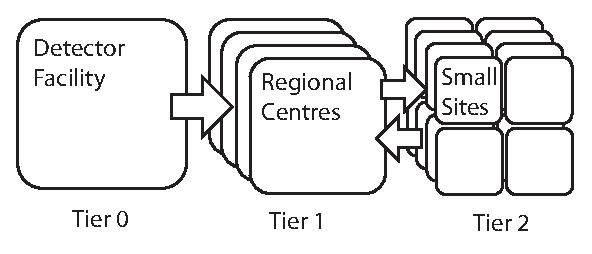
\includegraphics[width=3in]{tiered-data-flow.eps}
\caption{Schematic representation of the tiered data flow common to many HEP experiments. Raw and reconstructed detector data is produced at the detector facility and flows to regional centres, where it is safely stored, and large scale analyses are undertaken. Further processed data is transferred to smaller sites for smaller scale analyses; in addition, smaller sites produce simulated data of use to the whole collaboration which is cached at the regional centres.}
\end{figure}

Smaller persistent sites that are part of the core experiment infrastructure associate with the regional centres, just as the regional centres associate with the experimental centre. By associating sites in this way the load- in terms of resource access and network bandwidth- on the experimental centre is reduced. These smaller sites take part in more dynamic tasks, like the production of detector simulation data, or analysis of data already processed at the experimental centre.

The LHC computing era brings access to a dynamic infrastructure of sites that become part of a more dynamic Grid of resources. These smaller sites typically make resources available on something close to a best-effort basis- the extreme example being a physicist�s laptop. These resources are intended for rapidly changing analysis tasks, typically with much fewer resources (storage and bandwidth). This dynamic environment is more ideally suited to management by a grid that optimizes the storage and availability of data, and is driven by end-user analysis tasks.

The key problem is to seamlessly blend very high priority, continuous large-scale data transfers between highly available resources, with smaller scale, lower priority transfers between smaller sites for analysis, re-processing or re-analysis, and therefore make the infrastructure manageable by a small number of people. The data management layer needs to do this in an environment in which even the relatively static, stable core infrastructure is considered unreliable- and must therefore handle failover and retry of transfers to a given destination. It is also conceivable that high-priority transfers might get dynamically reallocated in the face of failure of a regional centre, guided by collaboration policy. 

The data management layer should provide sufficient functionality to allow a person or process to specify some group of files and a number of destinations, and then have the layer manage the efficient replication of data from wherever it currently resides to those destinations.

By devising a system in this manner, we meet the immediate needs of HEP experiments- which are typically the traditional large-scale directed transfers- by plugging in a simple replica management algorithm that takes subscriptions for datasets, and manages transfers as they become possible, without having a manager oversee the entire transfer process. We also make it possible to add to this simple replica management a more sophisticated optimizing replica manager as the system matures.

\section{Overall use cases for HEP data distribution}
In HEP there are two broad use cases for a data management layer: ``push" and ``stream" (or ``pull"). Push indicates the transfer of invaluable raw experimental data from the detector to tape store at regional centres. In this case, the collaboration chooses which regional centres store which data, and pushes the data onto them.

The streaming use case represents another on-going process instigated by either a regional centre, or a relatively stable smaller site. In this case, the site can subscribe to a given dataset; as files in this dataset are created, wherever they are created in the distribution infrastructure, they are transferred to the subscribing site. Similarly, these sites must make the data they create available for streaming to other sites.

The pull use case is a subset of stream, and represents a small-scale one-shot operation, in which say a single physicist is interested in some part of a dataset, and wishes to transfer it either to their University or even their laptop. In this case the end user would just connect their laptop or other resource to the data management layer, specify the data required, wait for the data management layer to transfer the necessary files and then remove the laptop from the layer.

Note that the names of these use cases are not intended to describe low-level transfer activity. In all cases we implement point to point transfers as third party- although in the majority of cases they are instigated by an agent running near the destination rather than the source.

The simplest requirements placed on the system are that it should be manageable at a high level by an individual, and that low level deployment and support take close to zero effort. To meet these requirements we devised an architecture based on quite simple, focused, robust processes that were able to handle failover and retry of transfers autonomously, and which could collaborate to solve the problem of transferring data over multiple hops to multiple destinations.

FIXME: Performance requirements ...

The system should also scale by the number of files in transfer. It should have a robust, internet-like design where no one part can bring entire transfer network down. The system should be able to saturate any hardware (network, storage) on which it is deployed. It should also operate completely asynchronously from other systems, for example: data management systems; data production processes; or analysis tasks running on batch computing nodes.

Within PhEDEx we have met, or will soon meet many of these requirements.

\section{Current PhEDEx architecture}
\subsection{Introduction}
HEP environments are typically heterogeneous at all levels of operation, although some standards in transfer tools and storage management are beginning to emerge. To develop PhEDEx we rely on a core set of tools and services that are most widely available. These tools and services are broadly cataegorized as part of storage management and transfer tools.

For storage management we rely on SRM (Storage Resource Management) \cite{srm:website}, which provides generic access to any storage resource. Superficially SRM provides a defined two step interaction through which a file can be obtained from any storage medium for which the user has a Storage URL (SURL), which contains the hostname of the medium. During an SRM transaction the client presents an SRM server with the SURL, is is returned a Transport URL (TURL) which indicates the current (possibly temporary) location of the file and a transport protocol that can be used to access it. This means that someone wishing to access a file at a given site does not need to know on which physical resource the file resides. 

Local file catalogues map some (collaboration level) global replica set identifer to some (local) identifer that can be used to access the file. These catalogues are not strictly seen as part of PhEDEx, as they are shared with other activities at each site- analysis tasks, for example.

A number of tools are used for point-to-point transfer of data. WAN transfers are made with tools that overlie gsiFTP \cite{gsiftp:website}- basically FTP with X509 certificate authentication. Such tools are globus-url-copy \cite{globus:website} and srmcp \cite{srmcp:website}. PhEDEx also uses a number of site-local transfer and tape management commands. This variety of tools is accomodated with a plug-in component design that allows the system to provide generic components that can be easily configured to use local tools when necessary.

\subsection{System design}
PhEDEx design and development is guided by a number of architectural principles. The key principle is that complex functionality should be kept in discrete units, and that the handover of responsibility for sections of the transfer workflow should be handed between those units using as few messages- containing minimal information- as possible \cite{paper:messaging}. As the system is active, with stateful components, it is reasonable to model these units after agents rather than as passive stateless services.

The PhEDEx design is characterised by layered abstractions. Our experience with data management tools has led us to view many operations and tools as unreliable. To manage this we wrap unreliable tools and systems in more robust layers to build a reliable data management system.

\begin{figure}
\centering
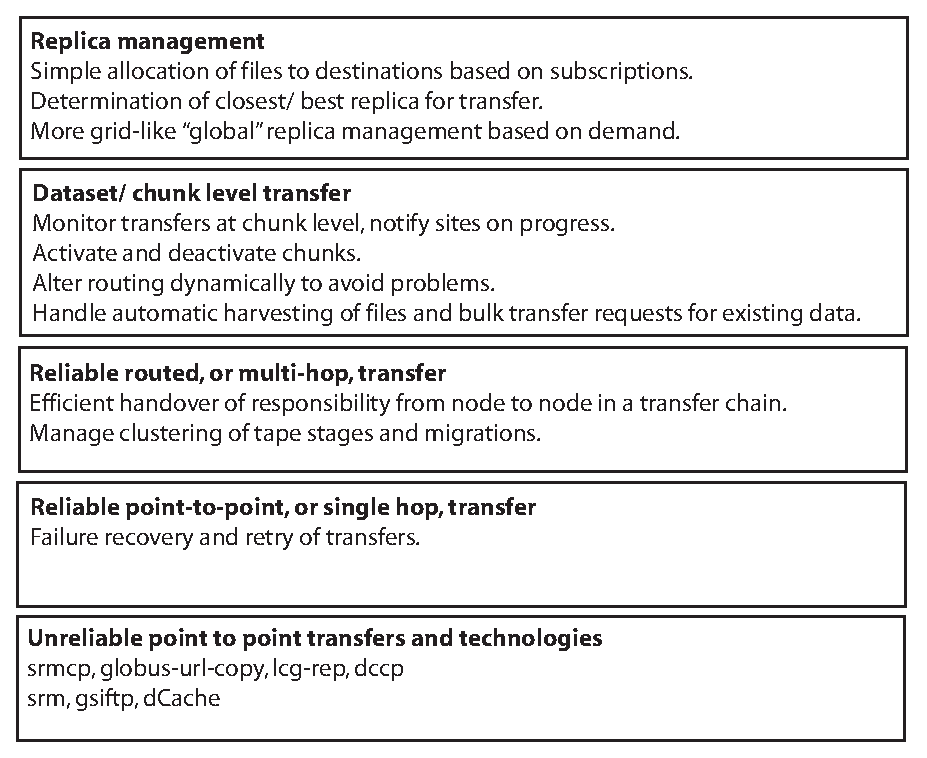
\includegraphics[width=3in]{phedex-layers.eps}
\caption{PhEDEx' layered architecture. Each layer is considered more reliable than the one below. For example: transfer tools are considered unreliable due to- in many cases- lack of reasonable failure recovery and unreliable error returns. The tools are therefore overlain by a layer that handles pre- and post-transfer validation checks and the subsequent retry of failed transfers. This layer also handles the collaboration between agents required to manage the clustered request and stage of data from tape, among other functions. }
\end{figure}

In addition, PhEDEx allows site managers to keep local information local, and allow as much local management of files as possible. This makes the system robust during local infrastructural change, but means that local and global information can become unsynchronised after deletion operations. For example, moving filesfrom one local disk to another is transparent if local catalogues are also kept up to date. However, file deletion requires an update of the PhEDEx system. This is not considered unscalable, as the straightforward deletion of files is rare in HEP systems: although data can be invalidated, it is rarely deleted. More problematic is the loss of files due to hardware failure; in this case PhEDEx currently relies on close interaction with local admin so that such failures are quickly accomodated.

To guide development we avoid creating services that aren't necessary, generally by accepting a small increase in complexity on the``client" transfer components. To make message passing simple we utilise a blackboard architecture in which transfer components post state information. The blackboard is currently deployed as a single high availability database. We also leverage data chunking to improve performance by avoiding somewhat traditional file-to-site mappings, instead mapping files to chunks and chunks to sites; we don't, however, require a chunk to exist anywhere in entirety.

\subsection{Overview of transfer operations}
The core element of the data management system is a node- a logical entity to which persistent processes named agents are associated. Typical examples might be a regional centre's transfer node, with agents to, for example, manage transfers from the centre's neighbours to the centre's disk buffers; or a mass storage node with an agent to manage the clustering of requests from other nodes for files for transfer.

Transfer workflows are divided into functionally coherent units- file transfer, for example, or migration to tape. Within those units workflow stages are defined as internal state transitions.  The handover of responsibility for a replication between units are seen as messages passed between agents, and are currently represented as state transitions on the blackboard. By way of example, the internal state transitions of a file transfer agent are: predelete, transfer, verify, postdelete, publish catalogue. The messages passed between agents involved in the transfer of files are for operations like: marking a number of files as wanted; or as being ready for transfer or migrate. This message passing represents the collaboration of agents to achieve their goals.

\begin{table}
\renewcommand{\arraystretch}{1.3}
\caption{Agent functionalities}
\centering
\begin{tabular}{c|p{2in}}
\hline
\bfseries Agent & \bfseries Description \\
\hline
\hline
Download & Manages the point to point transfer of files \\
Export & Manages the process of making files available on request by a Download agent \\
FileRouter & Triggers transfer hops for a given node based on nearest replica algorithm \\
NodeRouter & Maintains a node's routing table and contact with neighbours \\
\hline
\end{tabular}
\end{table}
FIXME: diagram of a typical agent workflow (internal, external state trans?)

The blackboard space that agents use to exchange messages/state information was envisaged as a database schema. This database schema provides us with a structure for defining a set of message ontologies, and its deployment as a database provides us with a reliable mechanism of communication. The information stored in this schema tracks the list of files currently of interest to the data management system, useful metadata concerning the nodes in the system (names, routing information) and high level subscription information (which sites subscribe to which datasets, and which files are currently allocated to which specific node). It also tracks the current state of point-to-point transfers, and maintains an RLI-like structure that maps global replica set identifiers to nodes in the distribution network.

Note that the database schema is designed with the goal of insulating information that is considered ``local": all tables are logically partitioned by node where possible, and agents typically only touch data concerning their own node, or that of their neighbours.

FIXME: overview schema diagram? 

Agents are defined at a high level only, in terms of their functional behaviour and expected interactions with other agents. They are developed using an agent toolkit, which wraps much of the low level functionality in common to all the agents: for example, handling database connections in a robust manner, or processing job queues. An explicit decision was made at the start of the project to wrap core message passing/ database access in a toolkit rather than to provide services that overlay the databases. 

The advantage of making agent code simpler through the deployment of services to handle chunks of complex functionality was deemed lower priority than the minimisation of maintenance and support effort required to maintain a performant service- especially when robust services to handle database interactions already exist: for example Oracle and MySQL both provide services to allow remote database interaction- to a large extent there is no need to create a new service over the top, however thin. This approach was taken in interactions with both the blackboard and, where possible, local file catalogues.

\section{Development, deployment and operations}
PhEDEx is currently deployed at 8 large CMS regional centres. It manages transfers between a variety of storage resource types: SRM, gsiftp servers, dCache \cite{dcache} disk pool managers, and a variety of underlying tape storage technologies (Castor \cite{castor}, Enstore \cite{enstore}, ADS \cite{ads}). WAN transfers are managed using globus-url-copy and srmcp.

The majority of the agents have been developed as perl scripts that call other transfer tools. Communication with other agents through the blackboard database is via wrapped client-side SQL.

As of February 2005 PhEDEx managed over 200TB of data. In the preceding 4 months it managed the transfer 45TB of data, with some sustained transfers of nearly 20TB a month. PhEDEx proved able to manage aggregate transfer rates in excess of 500 Mbps, including PhEDEx overhead for catalogue publishing and validation of transfers. Our current experience with the system is that efficient tape staging is the key bottleneck in the system: high rates can be achieved disk-to-disk, but stage pools are rapidly depleted of files to transfer. Generally the highest real stage rates achievable for tape stages are ~300Mbps; efficient tape stages represent the most keenly-sought improvement in our performance.

\section{Future developments}
Tender of contract for efficient file routing.

Explicit handling of "priority" at various granularities: what does priority mean, why do we need it, moving to priority based replica management (straightforward extension of simple scheduling/subscription replica management).

Queueing: filling trucks with parcels headed toward the same destination... simple attempts at this.

Peer to peer: what does it mean in this case; would it be useful? How close are we to this already? What information is global, which is local? What information might we accept a cost for/ sliding cost based on need?

Optimizing replica management? Coupling to workload management systems/ computational grids?

% Reminder: the "draftcls" or "draftclsnofoot", not "draft", class option
% should be used if it is desired that the figures are to be displayed while
% in draft mode.

% An example of a floating figure using the graphicx package.
% Note that \label must occur AFTER (or within) \caption.
% For figures, \caption should occur after the \includegraphics.
%
%\begin{figure}
%\centering
%\includegraphics[width=2.5in]{myfigure}
% where an .eps filename suffix will be assumed under latex, 
% and a .pdf suffix will be assumed for pdflatex
%\caption{Simulation Results}
%\label{fig_sim}
%\end{figure}


% An example of a double column floating figure using two subfigures.
%(The subfigure.sty package must be loaded for this to work.)
% The subfigure \label commands are set within each subfigure command, the
% \label for the overall fgure must come after \caption.
% \hfil must be used as a separator to get equal spacing
%
%\begin{figure*}
%\centerline{\subfigure[Case I]{\includegraphics[width=2.5in]{subfigcase1}
% where an .eps filename suffix will be assumed under latex, 
% and a .pdf suffix will be assumed for pdflatex
%\label{fig_first_case}}
%\hfil
%\subfigure[Case II]{\includegraphics[width=2.5in]{subfigcase2}
% where an .eps filename suffix will be assumed under latex, 
% and a .pdf suffix will be assumed for pdflatex
%\label{fig_second_case}}}
%\caption{Simulation results}
%\label{fig_sim}
%\end{figure*}



% An example of a floating table. Note that, for IEEE style tables, the 
% \caption command should come BEFORE the table. Table text will default to
% \footnotesize as IEEE normally uses this smaller font for tables.
% The \label must come after \caption as always.
%
%\begin{table}
%% increase table row spacing, adjust to taste
%\renewcommand{\arraystretch}{1.3}
%\caption{An Example of a Table}
%\label{table_example}
%\begin{center}
%% Some packages, such as MDW tools, offer better commands for making tables
%% than the plain LaTeX2e tabular which is used here.
%\begin{tabular}{|c||c|}
%\hline
%One & Two\\
%\hline
%Three & Four\\
%\hline
%\end{tabular}
%\end{center}
%\end{table}


\section{Conclusion}
The conclusion goes here.

% conference papers do not normally have an appendix

% use section* for acknowledgement
\section*{Acknowledgment}
% optional entry into table of contents (if used)
%\addcontentsline{toc}{section}{Acknowledgment}
The authors would like to thank...

% trigger a \newpage just before the given reference
% number - used to balance the columns on the last page
% adjust value as needed - may need to be readjusted if
% the document is modified later
%\IEEEtriggeratref{8}
% The "triggered" command can be changed if desired:
%\IEEEtriggercmd{\enlargethispage{-5in}}

% references section
% NOTE: BibTeX documentation can be easily obtained at:
% http://www.ctan.org/tex-archive/biblio/bibtex/contrib/doc/

% can use a bibliography generated by BibTeX as a .bbl file
% standard IEEE bibliography style from:
% http://www.ctan.org/tex-archive/macros/latex/contrib/supported/IEEEtran/bibtex
\bibliographystyle{IEEEtran.bst}
% argument is your BibTeX string definitions and bibliography database(s)
\bibliography{IEEEabrv,./barrass_et_al}
%
% <OR> manually copy in the resultant .bbl file
% set second argument of \begin to the number of references
% (used to reserve space for the reference number labels box)
%\begin{thebibliography}{1}

%\end{thebibliography}

% that's all folks
\end{document}


